\documentclass{beamer}


\graphicspath{ {pictures/} }

\usetheme{Boadilla}

\title{Distracted Driver Detection}
\subtitle{HLCV Project}
\author[Reyes, Schaefer, Tonsen, Weber]{Guillermo Reyes \\
	 Daniel Schaefer \\
	 Marc Tonsen \\
 Dominik Weber\\}
 \institute[]{Saarland University}
\date{11.07.2016}



\begin{document}
	\begin{frame}
		\titlepage
	\end{frame}
	
	
	\begin{frame}
		\frametitle{Task}
		Kaggle CV Competition: State Farm Distracted Driver Detection \\
		Given a picture of the driver predict the probability of the following classes:
		
		\begin{columns}
			\begin{column}{0.5\textwidth}
				\begin{itemize}
					\item c0: safe driving
					\item c1: texting - right
					\item c2: talking on the phone - right
					\item c3: texting - left
					\item c4: talking on the phone - left
					\item c5: operating the radio
					\item c6: drinking
					\item c7: reaching behind
					\item c8: hair and makeup
					\item c9: talking to passenger			
				\end{itemize}
			\end{column}
			\begin{column}{0.5\textwidth}  %%<--- here
				\begin{center}
					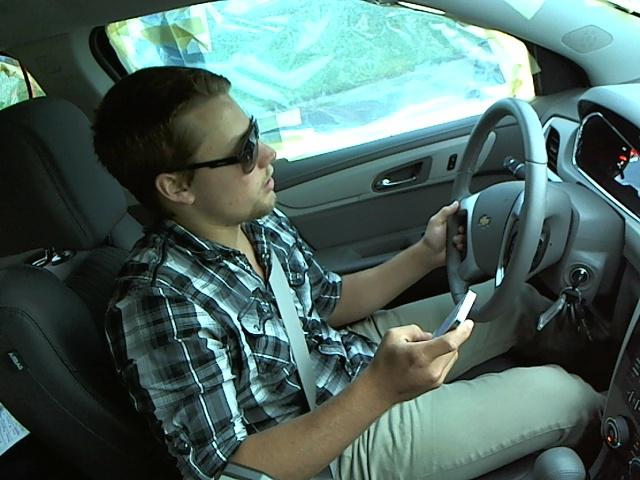
\includegraphics[width=0.9\textwidth]{img_6}
				\end{center}
			\end{column}
		\end{columns}
	\end{frame}

    \begin{frame}{theDataset}
        \frametitle{the Dataset}
        \begin{columns}
        \begin{column}{0.5\textwidth}
            \begin{itemize}
                \item around 2000 pictures per class
                    % in the available training set, which we also used for testing
                    % because we don't have the classes of the test set and we didn't
                    % want to rely on the online evaluation of the testset containing
                    % almost 80.000 pictures -> more control
                \item 26 different participants
                \item 4 different cars (with different camera angles)
                \item different light situations
                \item sometimes very minor differences between classes
             \end{itemize}
        \end{column}
        \begin{column}{0.5\textwidth}  %%<--- here
            \begin{center}
                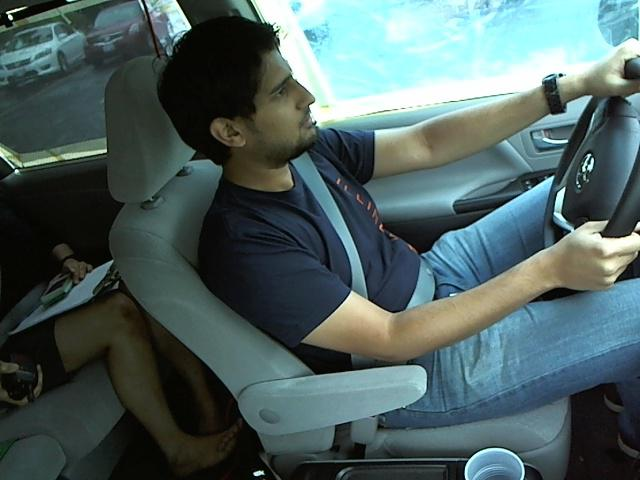
\includegraphics[width=0.8\textwidth]{c0}\\
                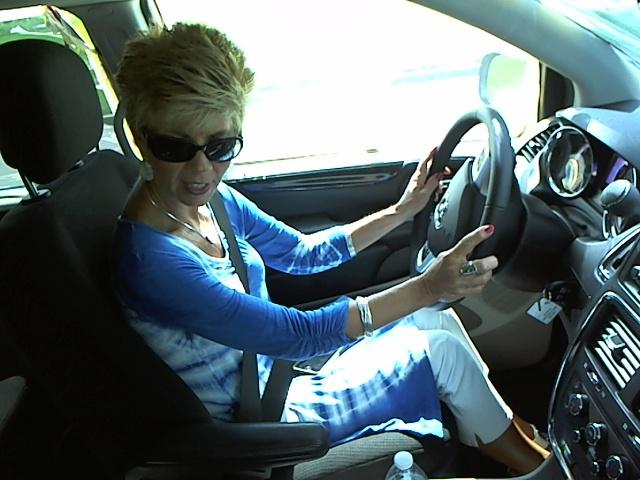
\includegraphics[width=0.8\textwidth]{c_0_angle2_passenger}
            \end{center}
        \end{column}
        \end{columns}
    \end{frame}
	
	
    
    
	\begin{frame}[allowframebreaks]
		\frametitle{References} 
		\nocite{*} 
		\bibliographystyle{amsalpha} 
		\bibliography{references} 
	\end{frame}
	
	\medskip

	
	
\end{document}
